% 第 15 题选项 D：F–x 先过原点线性上升、后跳变再线性上升的折线
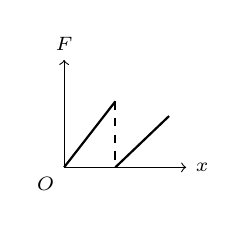
\begin{tikzpicture}[font=\scriptsize, scale=0.62]
  \draw[->] (0,0) -- (2.5,0) node[right] {$x$};
  \draw[->] (0,0) -- (0,2.2) node[above] {$F$};
  \node[below left] at (0,0) {$O$};
  \draw[thick] (0,0) -- (1.05,1.35);
  \draw[thick,dashed] (1.05,1.35) -- (1.05,0);
  \draw[thick] (1.05,0) -- (2.15,1.05);
\end{tikzpicture}
